

\section{Introduction}
A series of top cathode \gls{ito}\-/\gls{pedotpss}\-/\gls{mapi}\-/\gls{pcbm70}\-/\ch{Ag} perovskite solar cells have been fabricated.
The thickness of each of \gls{pedotpss} (\gls{htm}), \gls{mapi} (absorber), and \gls{pcbm70} (\gls{etm}) has been independently varied.
All these layers were deposited by spin coating and the thickness was tuned via spin coating speed.
These parameters where chosen so that their variation affect as little as possible the rest of the solar cell stack, so that we can unequivocally relate the observations to the changes.
%	\paragraph{The devices}
%The layers whose thickness was independently varied are the \gls{pedotpss} (\gls{htm}), the \gls{mapi} (absorber), and the \gls{pcbm70} (\gls{etm}).
The champion device performances of each configuration are listed in \cref{table:thicknesses_jv}.
The devices were fabricated and characterized by myself under the supervision of Dr.\ Nuria F.\ Montcada, Dr.\ Lydia Cabau, and Prof.\ Emilio J.\ Palomares Gil (fabrication described in \cpagerefrange{methods_top}{methods_top_end}).


\afterpage{
	%\begin{table}%[h]	% longtables cannot stay inside a float, otherwise they will not break
	\begin{xltabular}[c]{1.05\linewidth}{@{}>{\hsize=1.2\hsize}Y|>{\hsize=0.9\hsize}Y|>{\hsize=0.9\hsize}Y | c >{\hsize=1.5\hsize}Y >{\hsize=0.95\hsize}Y >{\hsize=0.75\hsize}Y >{\hsize=0.8\hsize}Y @{}}
		% multirow does not get the correct number of rows with tabularx
		% mycaption does not work inside xltabular
		\caption[Layers thicknesses and related average performances of top cathode cells.]{\textbf{Layers thicknesses and related average performances of top cathode cells.}
			Explored thicknesses with \textit{average} forward and reverse J-V sweep performances.
			The standard deviation for each value is indicated after the $\pm$ symbol.
			For each reported result, at least 8, 8, and 4 devices were averaged respectively for \gls{mapi}, \gls{pcbm70}, and \gls{pedotpss} thickness exploration.
			\Gls{etm} column indicates the \gls{pcbm70} thickness, while \gls{htm} one refers to \gls{pedotpss} thickness.
			The measurement conditions were \SI{1}{sun} illumination, no light soaking, \SI{1}{\V\per\s} sweep speed.
			A boxplot representation of this data can be found in \authoryear{Gelmetti2017}.
			J-V curve for record devices are reported in \cref{fig:jv_champions-mapi,fig:jv_champions-pcbm,fig:jv_champions-pedotpss}.
		}\label{table:thicknesses_jv}\\[\belowcaptionskip]
		\multicolumn3{c|}{\small\textbf{Layers thickness}} & \multicolumn{5}{c}{\small\textbf{J-V sweep parameters}}
		\rule[-1ex]{0pt}{3ex} \\
		\small\gls{mapi} &  \small\gls{etm} & \small\gls{htm} &\small Sweep & \small\gls{jsc} &  \small\gls{voc} & \small\gls{ff} &  \small\gls{pce} \\ 
		\rule[-1ex]{0pt}{2.5ex}  \footnotesize\si{\nm} &  \footnotesize\si{\nm} &  \footnotesize\si{\nm} & - & \footnotesize\si{\mA\per\square\cm} &  \footnotesize\si{\V} & \footnotesize\si{\%} &  \footnotesize\si{\%} \\[1mm]
		\hline
		\endfirsthead
		\multicolumn{2}{@{}l}{\ldots \small continues}\\
		\hline
		\small\gls{mapi} & \small\gls{etm} & \small\gls{htm} &\small Sweep & \small\gls{jsc} & \small\gls{voc} & \small\gls{ff} & \small\gls{pce} \\ 
		\hline
		\endhead
		\hline
		\multicolumn{8}{r@{}}{\small continues\ldots}\\
		\endfoot
		\hline
		\endlastfoot
		\rule[-1ex]{0pt}{3ex}
		\multirow{3}{*}{230} 	& \multirow{11}{*}{40}	&  \multirow{11}{*}{65}	&fwd	&	13.5	$\pm	0.5	$ & 	1.03	$\pm	0.01	$ & 	53	$\pm	3	$ & 	7.3	$\pm	0.4	$ \\*
		\rule[-1ex]{0pt}{2.5ex}
		&  						& 						&rev	&	13.6	$\pm	0.5	$ & 	1.02	$\pm	0.01	$ & 	55	$\pm	3	$ & 	7.7	$\pm	0.5	$ \\*
		\cline{1-1} \cline{4-8}
		\multirow{3}{*}{320}	&  						&  						&fwd	&	13.9	$\pm	0.3	$ & 	1.04	$\pm	0.01	$ & 	57	$\pm	5	$ & 	8.2	$\pm	0.6	$ \\*
		\rule[-1ex]{0pt}{2.5ex}
		&  						&  						&rev	&	14.1	$\pm	0.3	$ & 	1.04	$\pm	0.01	$ & 	55	$\pm	4	$ & 	8.1	$\pm	0.5	$ \\*
		\cline{1-1} \cline{4-8}
		\multirow{3}{*}{440}	&  						&  						&fwd	&	16.3	$\pm	2.1	$ & 	1.01	$\pm	0.04	$ & 	58	$\pm	2	$ & 	9.5	$\pm	0.8	$ \\*
		\rule[-1ex]{0pt}{2.5ex}
		&  						&  						&rev	&	16.5	$\pm	1.9	$ & 	0.98	$\pm	0.07	$ & 	50	$\pm	5	$ & 	8.1	$\pm	1.4	$ \\[1mm]
		\hline
		\multirow{15}{*}{350}	& \multirow{3}{*}{40} 	&  \multirow{15}{*}{65} &fwd	&	16.4	$\pm	2.2	$ & 	0.93	$\pm	0.06	$ & 	48	$\pm	8	$ & 	7.4	$\pm	1.8	$ \\*
		&  						&  						&rev	&	16.1	$\pm	2.1	$ & 	0.95	$\pm	0.06	$ & 	50	$\pm	5	$ & 	7.6	$\pm	1.4	$ \\*
		\cline{2-2} \cline{4-8}
		& \multirow{3}{*}{60} 	& 					 	&fwd	&	13.2	$\pm	1.1	$ & 	0.99	$\pm	0.04	$ & 	47	$\pm	6	$ & 	6.2	$\pm	1.1	$ \\*
		&  						&  						&rev	&	12.8	$\pm	0.7	$ & 	0.98	$\pm	0.05	$ & 	47	$\pm	5	$ & 	5.9	$\pm	0.8	$ \\*
		\cline{2-2} \cline{4-8}
		& \multirow{3}{*}{90} 	&  						&fwd	&	11.1	$\pm	0.6	$ & 	1.03	$\pm	0.03	$ & 	42	$\pm	2	$ & 	4.8	$\pm	0.6	$ \\*
		&  						&  						&rev	&	11.1	$\pm	0.8	$ & 	1.00	$\pm	0.04	$ & 	44	$\pm	2	$ & 	4.8	$\pm	0.5	$ \\*
		\cline{2-2} \cline{4-8}
		& \multirow{3}{*}{120} 	&  						&fwd	&	7.7	$\pm	1.6	$ & 	1.02	$\pm	0.04	$ & 	18	$\pm	2	$ & 	1.4	$\pm	0.4	$ \\*
		&  						&  						&rev	&	7.6	$\pm	1.6	$ & 	1.01	$\pm	0.04	$ & 	18	$\pm	2	$ & 	1.4	$\pm	0.4	$ \\[1mm]
		\hline
		\multirow{11}{*}{300}	& \multirow{11}{*}{40}	& \multirow{3}{*}{27} 	&fwd	&	12.3	$\pm	1.5	$ & 	1.04	$\pm	0.03	$ & 	55	$\pm	9	$ & 	6.9	$\pm	0.8	$ \\*
		&  						&  						&rev	&	11.9	$\pm	1.7	$ & 	1.03	$\pm	0.04	$ & 	54	$\pm	11	$ & 	6.6	$\pm	0.7	$ \\*
		\cline{3-8}
		&  						& \multirow{3}{*}{45} 	&fwd	&	12.2	$\pm	1.7	$ & 	1.04	$\pm	0.01	$ & 	58	$\pm	4	$ & 	7.3	$\pm	1.2	$ \\*
		&  						&  						&rev	&	11.8	$\pm	1.7	$ & 	1.00	$\pm	0.09	$ & 	53	$\pm	7	$ & 	6.2	$\pm	0.9	$ \\*
		\cline{3-8}
		& 				 		& \multirow{3}{*}{65} 	&fwd	&	12.4	$\pm	1.6	$ & 	1.04	$\pm	0.02	$ & 	60	$\pm	3	$ & 	7.7	$\pm	0.6	$ \\*
		&  						&  						&rev	&	12.6	$\pm	1.4	$ & 	1.00	$\pm	0.10	$ & 	60	$\pm	4	$ & 	7.5	$\pm	0.4	$ \\[1mm]
	\end{xltabular}
}



\section{Design of the Experiment}
	Perovskite synthesis is a very easy and fragile process at the same time.
	When varying a fabrication parameter, for example during an optimization, it is quite likely to provoke a "butterfly effect" with the resulting device differing from the reference by much more than the characteristic under study.
	A principal component analysis of the fabrication parameters would be needed for a rational optimization, but such a complex procedure is further hindered by the difficulty of identifying all relevant contributions.
	In this study we vary a set of parameters that hopefully have a foreseeable relation with the resulting device structure: thickness of each layer, through the tuning of the spin coating deposition speed.
This variation should just affect the thickness of one layer, having just a minor influence on the other layers and the rest of the device physical features.
This will allow us to univocally relate the observations to the modifications.


\section{Varying \glsentrytext{mapi} Thickness (Absorber Layer)}

\begin{figure}
	\makebox[\textwidth][c]{
		\parbox{1.1\textwidth}{
			\centering
			\begin{subfigure}[t]{0.51\textwidth}
				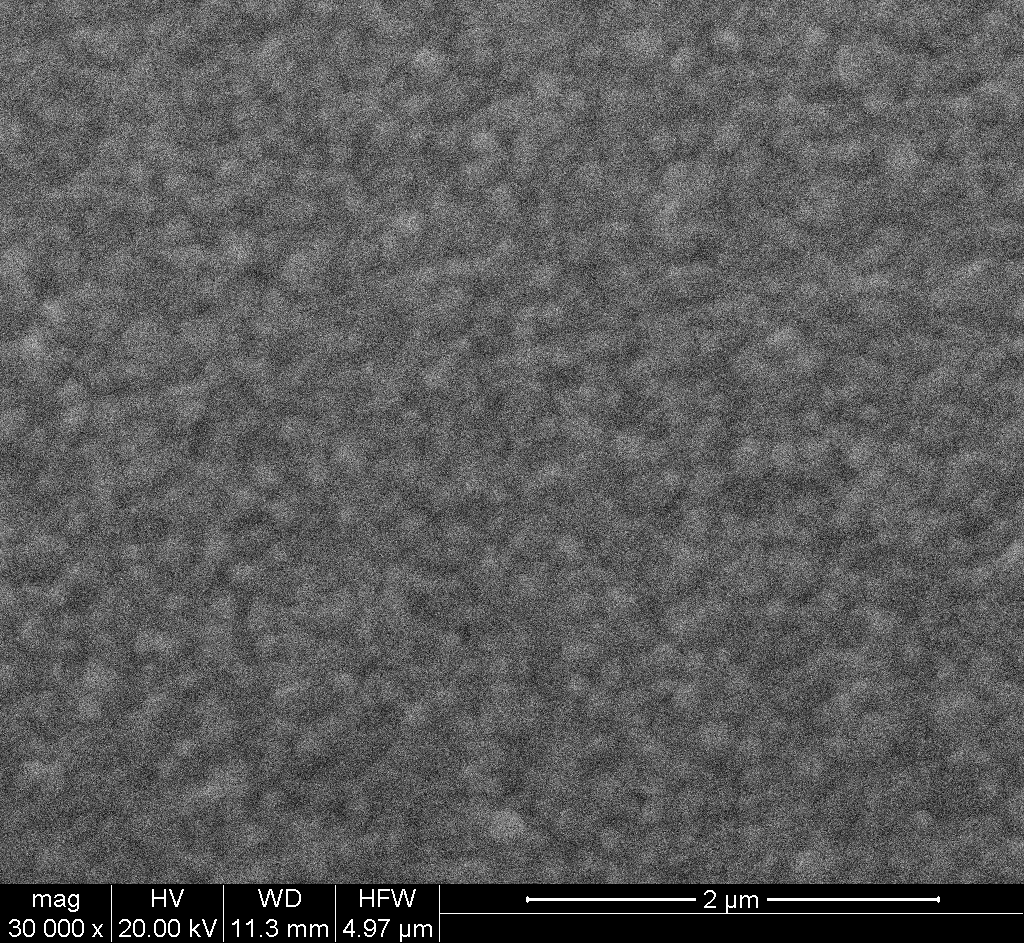
\includegraphics[width=1\textwidth]{esem-topview/ig87-c39-8000RPM-30k-hv-contrast.png}
				\subcaption{\SI{8000}{\rpm}, \SI{230}{\nm}}\label{fig:thicknesses-esem-topview-8000RPM}
			\end{subfigure}
			\qquad
			\begin{subfigure}[t]{0.51\textwidth}
				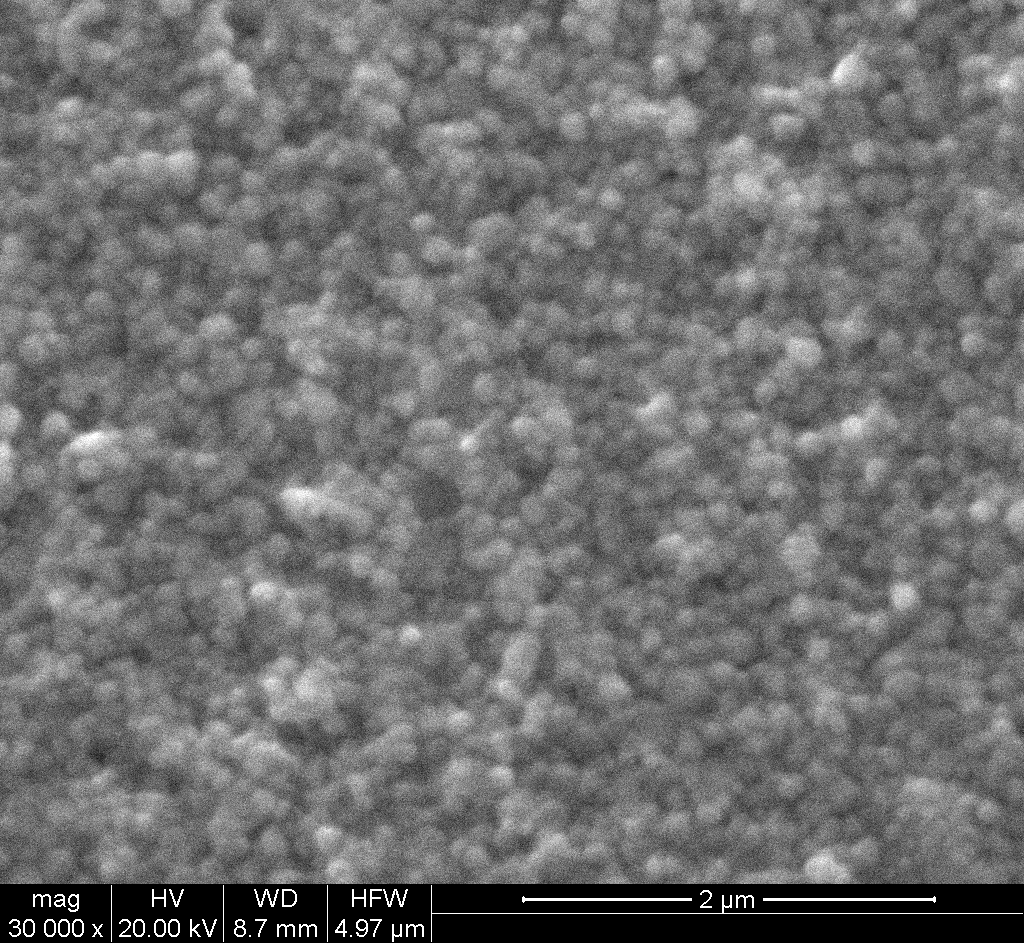
\includegraphics[width=1\textwidth]{esem-topview/ig87-b78-4100RPM-30k-hv-contrast.png}
				\subcaption{\SI{4100}{\rpm}, \SI{320}{\nm}}\label{fig:thicknesses-esem-topview-4100RPM}
			\end{subfigure}
			\bigskip
			
			\begin{subfigure}[t]{0.51\textwidth}
				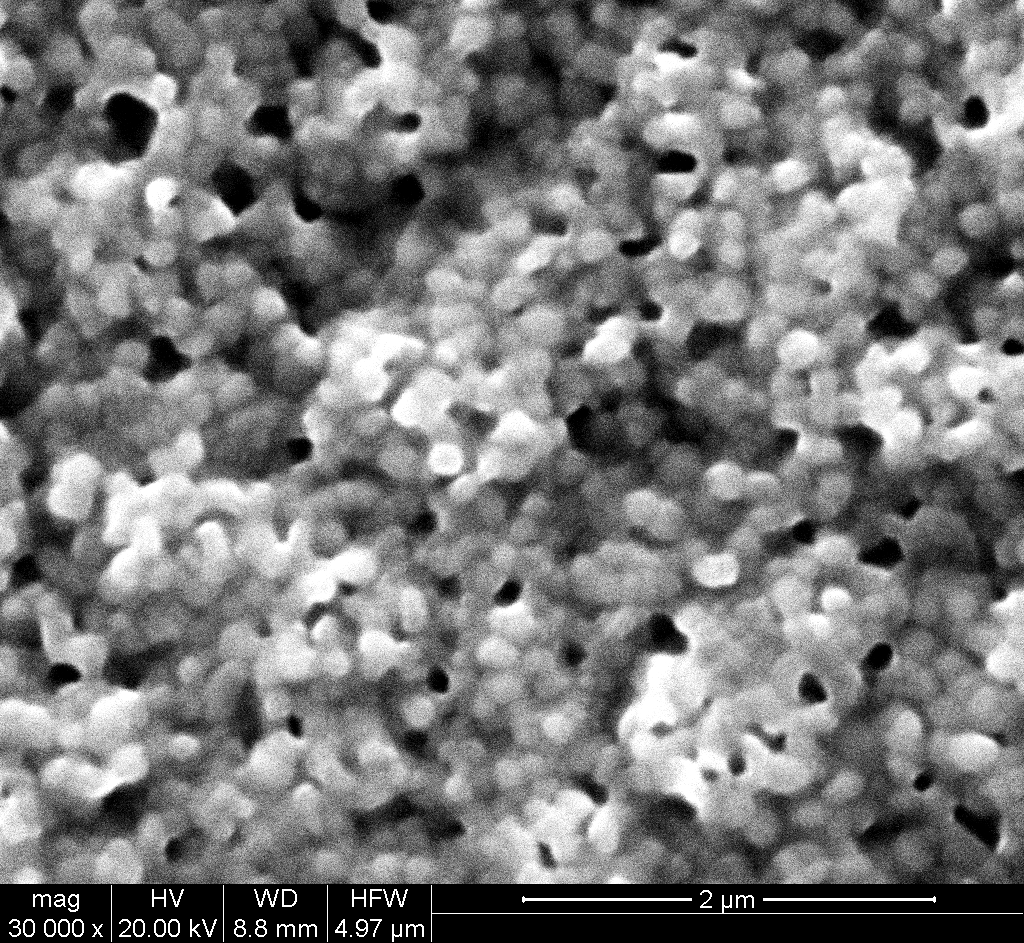
\includegraphics[width=1\textwidth]{esem-topview/ig87-c34-2000RPM-30k-hv-contrast.png}
				\subcaption{\SI{2000}{\rpm}, \SI{440}{\nm}}\label{fig:thicknesseses-esem-topview-2000RPM}
			\end{subfigure}
			\mycaption[Top view ESEM images of annealed perovskite layers with various thicknesses.]{The surface of a thin perovskite layer is studied using  FIJI/ImageJ \cite{Schindelin2012} on images of two different devices for each deposition condition (just one reported here for brevity). The average domain diameter and its standard deviation in parenthesis is \SI{182 \pm 25}{\nm} for the thin \SI{230}{\nm} perovskite layer in (\textbf{a}), \SI{190 \pm 34}{\nm} for the medium \SI{320}{\nm} perovskite layer in (\textbf{b}), \SI{189 \pm 23}{\nm} for the thick \SI{440}{\nm} perovskite layer in (\textbf{c}).}\label{fig:thicknesses-esem-topview}
		}
	}
\end{figure}

\paragraph{Roughness and grain size}
Using different spin coating speeds, devices with various \gls{mapi} thicknesses were obtained, as detailed in \cref{table:mapi_thickness}.
As a consequence to the different deposition conditions, the \gls{mapi} surface is more rough for the thick device than for the thin one, as can be intuited looking at \gls{esem} image in \cref{fig:thicknesses-esem-topview}.
Any way, measuring the roughness average with a profilometer, it resulted to be \SI{< 10}{\nm} for all the cases, so the \SI{40}{\nm} \gls{pcbm70} layer should be enough for an homogeneous coverage.
From the same \gls{esem} image, we can measure the grain lateral size, which is not significantly different for the six observed samples (two per each \gls{mapi} thickness, data detailed in \cref{fig:thicknesses-esem-topview} caption).

\begin{SCfigure}
	\centering
	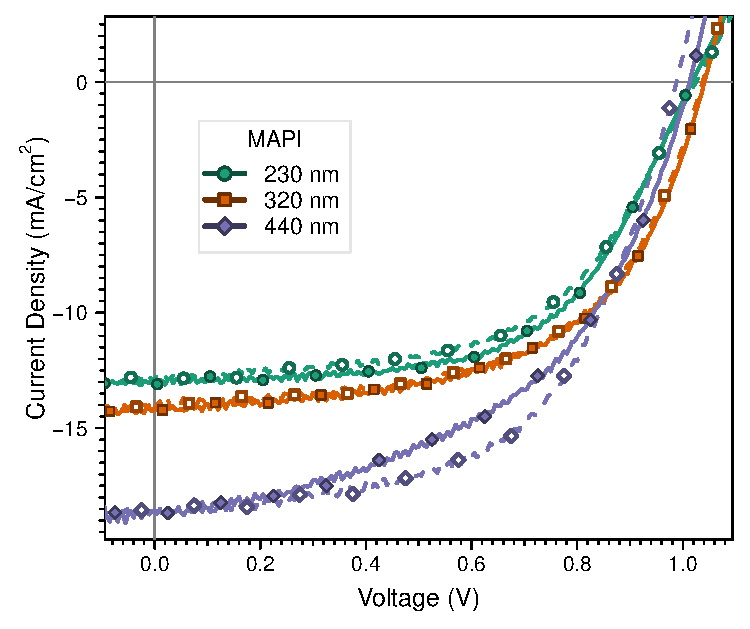
\includegraphics[width=0.8\textwidth]{jv_champions-mapi/mapi-IVs.pdf}
	\mycaption[Current-voltage sweeps for champion devices with different MAPI thicknesses.]{The solid line with filled markers represents the forward scan, while the dashed line with hollow markers represents the reverse scan.}\label{fig:thicknesses-jv_champions-mapi}
\end{SCfigure}

\paragraph{Current-voltage sweeps}
In \cref{fig:thicknesses-jv_champions-mapi} we can observe the current-voltage sweeps of the champion devices while in \cref{table:thicknesses_jv} the averages and standard deviations are reported.
%\paragraph{Current-voltage sweeps -- \gls{ff}}
The \gls{ff} is not significantly different for the devices with different \gls{mapi} layer thickness.
The only observable difference is the presence of a higher hysteresis (difference between forward and reverse scan) in this parameter for the thicker \gls{mapi} case.
This could indicate a small change in the perovskite\-/\gls{pcbm70} interface or just a change in the hysteresis characteristic time due to the increased ionic resistance in the thicker \gls{mapi} layer. 
%\paragraph{Current-voltage sweeps -- \gls{voc}}
Regarding the \gls{voc}, this value also did not change with thickness, indicating that the same recombination processes and dynamics are present disregarding the absorber thickness.
The higher deviation of this parameter for the thicker perovskite could be due to its higher roughness, causing some devices to have pinholes in the \gls{etm} layer.
%\paragraph{Current-voltage sweeps -- \gls{jsc} and \gls{pce}}
What is clear and expected is the \gls{jsc} increase.
This is most likely due to the low \gls{eqe} in the thin perovskite layer due to its far\hyp{}from\hyp{}zero transmittance.
The increase in photogeneration rate is reflected in an increase of \gls{pce}.

\afterpage{
%\begin{table}%[h]	% longtables cannot stay inside a float, if they do, they will not break
\begin{xltabular}[c]{1.05\linewidth}{@{} >{\hsize=1.1\hsize}Y | >{\hsize=0.7\hsize}Y | >{\hsize=0.7\hsize}Y | Y >{\hsize=1.65\hsize}Y >{\hsize=0.6\hsize}Y | Y  >{\hsize=1.65\hsize}Y >{\hsize=0.6\hsize}Y @{}}
	% multirow does not get the correct number of rows with tabularx
	% mycaption does not work inside xltabular
	\caption[Parameters fitted from CE and DC data, from devices with different layers' thicknesses.]{\textbf{Parameters fitted from CE and DC data, from devices with different layers' thicknesses.}
		 The experimental data reported in \cref{fig:thicknesses-mapi-geometric,fig:thicknesses-pcbm-geometric,fig:thicknesses-pedotpss-geometric} has been fitted using \cref{eq:ce_full} for \gls{ce} data and \cref{eq:dc_full} for \gls{dc} data.
	}\label{table:thicknesses_photophysics}\\[\belowcaptionskip]
	\multicolumn3{c|}{\small\textbf{Layers thickness}} & \multicolumn{3}{c|}{\small\textbf{CE}} & \multicolumn{3}{c}{\small\textbf{DC}}
	\rule[-1ex]{0pt}{3ex} \\
	\small\gls{mapi} &  \small\gls{etm} & \small\gls{htm} & \small\gls{symb:Cg} & \small\gls{symb:neq} &  \small\gls{symb:m} & \small\gls{symb:Cg} & \small\gls{symb:neq} &  \small\gls{symb:m} \\ 
	\rule[-1ex]{0pt}{2.5ex}  \footnotesize\si{\nm} &  \footnotesize\si{\nm} &  \footnotesize\si{\nm} & \footnotesize\si{\nano\F\per\square\cm} &  \footnotesize\si{\coulomb\per\square\cm} & - &  \footnotesize\si{\nano\F\per\square\cm} &  \footnotesize\si{\coulomb\per\square\cm} & - \\[1mm]
	\hline
	\endfirsthead
	\multicolumn{2}{@{}l}{\ldots \small continues}\\
	\hline
	\small\gls{mapi} & \small\gls{etm} & \small\gls{htm} & \small\gls{symb:Cg} & \small\gls{symb:neq} & \small\gls{symb:m} & \small\gls{symb:Cg} & \small\gls{symb:neq} & \small\gls{symb:m} \\ 
	\hline
	\endhead
	\hline
	\multicolumn{9}{r@{}}{\small continues\ldots}\\
	\endfoot
	\hline
	\endlastfoot
	\rule[-1ex]{0pt}{4ex}
	230 	& \multirow{3}{*}{40}	&  \multirow{3}{*}{65}	& \rnum{85.3301567640111}	& \rnum{5.12603766463996e-21}	& \rnum{1.42540882502849}	& \rnum{63.5691599645725}	& \rnum{2.80156436794216e-12}	& \rnum{4.42885311532801} \\*
	\cline{1-1} \cline{4-9}
\rule[-1ex]{0pt}{4ex}
	320	&  						& 						& \rnum{77.7280226931573}	& \rnum{4.82359451755698e-27}	& \rnum{0.970504332684817}	& \rnum{55.4099677743798}	& \rnum{9.01531708758845e-13}	& \rnum{4.09817044704697} \\*
	\cline{1-1} \cline{4-9}
	\rule[-1ex]{0pt}{4ex}
440	&  						& 						& \rnum{70.7196355753457}	& \rnum{1.1916876016195e-27}	& \rnum{0.912575007143644}	& \rnum{50.42918432699}	& \rnum{8.6536760550073e-15}	& \rnum{2.64532408455481} \\
	\hline
	\rule[-1ex]{0pt}{4ex}
	\multirow{3}{*}{350}	& 40 	&  \multirow{3}{*}{65} & \rnum{76.399963266735} & \rnum{2.59099124009742e-20} & \rnum{1.42377526492346} & \rnum{55.0987488891515} & \rnum{7.87748762963633e-15} & \rnum{2.51025076329765}\\*
	\cline{2-2} \cline{4-9}
	\rule[-1ex]{0pt}{4ex}
							& 60 	& 					 	& \rnum{61.3214241914314} & \rnum{9.01470965786247e-25} & \rnum{1.07005213324604} & \rnum{42.8290117954868} & \rnum{9.34331162626908e-13} & \rnum{3.81783541577789} \\*
	\cline{2-2} \cline{4-9}
	\rule[-1ex]{0pt}{4ex}
							& 90 	&  						&\rnum{43.8300398524054} & \rnum{5.33438024104082e-29} & \rnum{0.853781763130922} & \rnum{33.9400710508692} & \rnum{4.49280198629451e-11} & \rnum{5.98365652726317}\\
	\hline
	\rule[-1ex]{0pt}{4ex}
	\multirow{3}{*}{300}	& \multirow{3}{*}{40}	& 27 	& \rnum{63.8554990179897} & \rnum{9.74708581977915e-15} & \rnum{2.93729998552211} & \rnum{46.1396721657447} & \rnum{1.63620664547478e-15} & \rnum{2.37232492243424}\\*
	\cline{3-9}
	\rule[-1ex]{0pt}{4ex}
							&  						& 45	& \rnum{66.7217372609922} & \rnum{6.39620737296978e-21} & \rnum{1.2951381459487} & \rnum{49.8531675841145} & \rnum{4.64793103413763e-16} & \rnum{2.13846267623868} \\*
	\cline{3-9}
	\rule[-1ex]{0pt}{4ex}
							& 				 		& 65	& \rnum{64.4501923191207} & \rnum{5.44744643856892e-32} & \rnum{0.678974589798595} & \rnum{50.3194494652546} & \rnum{1.34432980262899e-16} & \rnum{2.00044590997543}\\
\end{xltabular}
%\end{table}
}

\paragraph{Geometric capacitance from \gls{dc} and \gls{ce}}
From the low and mid background light capacitance obtained from \gls{dc} in \cref{fig:thicknesses-mapi-geometric-dc} and from the linear part of \gls{ce} in \cref{fig:thicknesses-mapi-geometric-ce} we can obtain a geometric capacitance $C_|g|$, as explained in \cref{ch:characterization}.
This capacitance arises from the accumulation of charges in the selective contacts' depletion layers, considering this as a parallel plates capacitor it's easy to foresee that the increase of \gls{mapi} layer will increase the distance between the "plates" and cause a decrease in the capacitance.
Please note that this is valid just if the \gls{ce} is integrated over short times, so that the ionic displacement is negligible.
Otherwise, as explained in AAAAAAAAAAAAAAAAAAAAAAAAAAA, the measured geometric capacitance would regard charges (ionic and electronic) accumulating on the two sides of each perovskite\-/contact interface (a junction capacitance rather than a geometric capacitance), being insensitive to the \gls{mapi} thickness.
%This can be observed from the tilting of the linear regime of charge \textsl{versus} light bias  or in the constant capacitance regime .
The fitted values of $C_|g|$ are reported in \cref{table:thicknesses_photophysics}.

\begin{figure}
	\makebox[\textwidth][c]{
		\parbox{1.1\textwidth}{
			\centering
			\begin{subfigure}[t]{0.51\textwidth}
				\includegraphics[width=1\textwidth]{photophysics-mapi/photophysics-CEs.pdf}
				\subcaption{Charge from \gls{ce}}\label{fig:thicknesses-mapi-geometric-ce}
			\end{subfigure}
			\qquad
			\begin{subfigure}[t]{0.51\textwidth}
				\includegraphics[width=1\textwidth]{photophysics-mapi/photophysics-DCs-capacitance.pdf}
				\subcaption{Capacitance from \gls{dc}}\label{fig:thicknesses-mapi-geometric-dc}
			\end{subfigure}
			\mycaption[CE and DC of devices with different MAPI thicknesses, highlighting the varying geometric capacitance.]{
				In (\textbf{a}) the charge \textsl{versus} light bias as obtained from \gls{ce} is reported. The dark solid line is an exponential fitting following \cref{eq:ce_full} while the light solid line reports just its exponential addend, ignoring the geometric capacitance. In (\textbf{b}) the capacitance dependence on light bias is reported as obtained from \gls{dc}. The solid line indicates the fitting using \cref{eq:dc_full}. All the fitted parameters are reported in \cref{table:thicknesses_photophysics}.
			}\label{fig:thicknesses-mapi-geometric}
		}
	}
\end{figure}

%\paragraph{Exponential charge distribution from \gls{dc} and \gls{ce}}
%Both from \gls{ce} in \cref{fig:thicknesses-mapi-geometric-ce} and from \gls{dc} in \cref{fig:thicknesses-mapi-geometric-dc} we can see that the exponential regime in the charge accumulation, assigned to the chemical capacitance of charges accumulating in the perovskite layer, is similar for all the thicknesses.
%Indeed, no change was expected as the energy levels of the layers is identical in all the devices.
%Additionally, comparing the two techniques' results for the same sample, we can notice that in every case the exponential regimes starts at lower voltages for \gls{dc}.
%This discrepancy between the two techniques is not always observed for perovskite solar cells and its interpretation is pending.

%\paragraph{Carriers life-time}
%Then we studied the carriers life-time \textsl{via} \gls{tpv} and related these to the chemical charge (subtracting the charges stored in the geometric capacitance) obtained either \textsl{via} \gls{ce} or \textsl{via} \gls{dc} we can confirm 
%
%\begin{figure}
%	\makebox[\textwidth][c]{
%		\parbox{1.1\textwidth}{
%			\centering
%			\begin{subfigure}[t]{0.51\textwidth}
%				\includegraphics[width=1\textwidth]{photophysics-mapi/photophysics-TPVCEs-nogeom_total.pdf}
%				\subcaption{\Gls{tpv} life-time \textsl{versus} \gls{ce} charge}\label{fig:thicknesses-mapi-tpv-ce}
%			\end{subfigure}
%			\qquad
%			\begin{subfigure}[t]{0.51\textwidth}
%				\includegraphics[width=1\textwidth]{photophysics-mapi/photophysics-TPVDCs-nogeom_total.pdf}
%				\subcaption{\Gls{tpv} life-time \textsl{versus} \gls{dc} charge}\label{fig:thicknesses-mapi-tpv-dc}
%			\end{subfigure}
%			\mycaption[Total carrier life-time \textsl{versus} charge of devices with different MAPI thicknesses.]{The small perturbation life-times were obtained \textsl{via} \gls{tpv} and corrected to total carrier life-time as reported in \cref{eq:tau_pfo}. In (\textbf{a}) the recombination orders needed for the correction were obtained from the fitting the small perturbation life-time \textsl{versus} chemical charge from \gls{ce}, while in (\textbf{b}) the chemical charge from \gls{dc} was used. Additionally, in (\textbf{a}) the chemical charge \textsl{versus} light bias needed for the $x$~axis, was taken from \gls{ce}, while in (\textbf{b}) it was obtained from \gls{dc}.}\label{fig:thicknesses-mapi-tpv}
%		}
%	}
%\end{figure}

\section{Varying \glsentrytext{pcbm70} Thickness (\glsentryshort{etm} Layer)}
Using different spin coating speeds, devices with various \gls{pcbm70} thicknesses were obtained, as detailed in \cref{table:pcbm_thickness}.
This was deposited on top of a rather thin layer of \SI{350}{\nm} of \gls{mapi}, which resulted to be smooth enough to allow the \gls{pcbm70} to homogeneously cover it.

\begin{SCfigure}
	\centering
	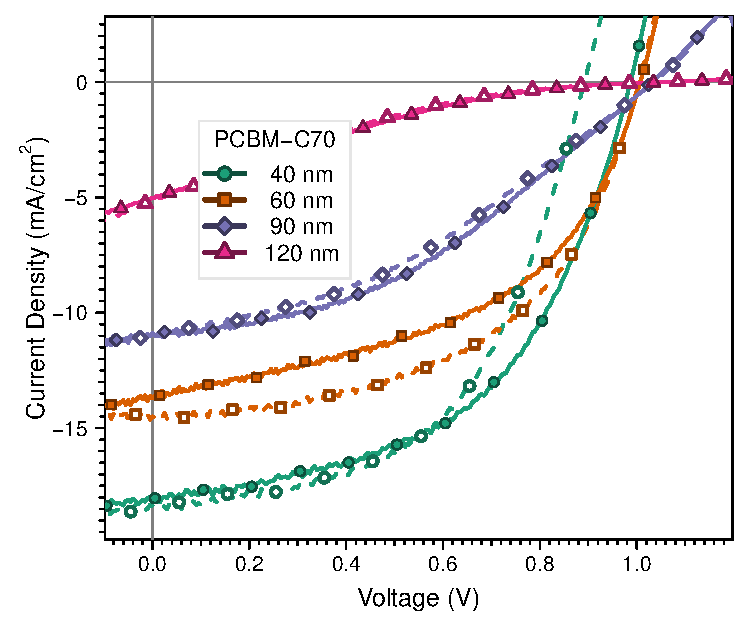
\includegraphics[width=0.8\textwidth]{jv_champions-pcbm/pcbm-IVs.pdf}
	\mycaption[Current-voltage sweeps for champion devices with different \glsentrytext{pcbm70} thicknesses.]{The solid line with filled markers represents the forward scan, while the dashed line with hollow markers represents the reverse scan.}\label{fig:thicknesses-jv_champions-pcbm}
\end{SCfigure}

\paragraph{Current-voltage sweeps}
In \cref{fig:thicknesses-jv_champions-pcbm} we can observe the current-voltage sweeps of the champion devices while in \cref{table:thicknesses_jv} the averages and standard deviations are reported.
%\paragraph{Current-voltage sweeps -- \gls{ff}}
The \gls{ff} is heavily affected by the high series resistance of the thicker \gls{pcbm70} layer.
The S-shape observed close to \gls{voc} in the current\hyp{}voltage sweep of devices with thick \gls{etm} layer is due to the poor mobility of electrons in \gls{pcbm70} \cite{VonHauff2005} which causes a charges collection bottleneck \cite{Wheeler2015}. 
%\paragraph{Current-voltage sweeps -- \gls{voc}}
Interestingly enough, the \gls{voc} slightly increases when the \gls{pcbm70} thickness is increased.
If confirmed with a stronger statistics, the lower voltage for the thinner layer case could be explained by the presence of some uncovered perovskite area, causing a leakage current between the perovskite and the silver metal electrode.
%\paragraph{Current-voltage sweeps -- \gls{jsc} and \gls{pce}}
As also observed by \authoryear{Seo2014}, increasing the \gls{pcbm70} layer results in a strong decrease of the \gls{jsc}.
In \authoryear{Shao2016}, the same dependency is observed in disordered \gls{pcbm70} films while it is not present if the layer is solvent annealed.
Indeed, a very large series resistance, caused by the thick \gls{etm} layer, is expected to affect the short circuit current (this can be seen substituting $V=0$ in the implicit function in \cref{eq:series_resistance}).
This influence, together with the higher \gls{ff} results in a much higher \gls{pce} for devices with a thin \gls{etm}.

\begin{figure}
	\makebox[\textwidth][c]{
		\parbox{1.1\textwidth}{
			\centering
			\begin{subfigure}[t]{0.51\textwidth}
				\includegraphics[width=1\textwidth]{photophysics-pcbm/photophysics-CEs.pdf}
				\subcaption{Charge from \gls{ce}}\label{fig:thicknesses-pcbm-geometric-ce}
			\end{subfigure}
			\qquad
			\begin{subfigure}[t]{0.51\textwidth}
				\includegraphics[width=1\textwidth]{photophysics-pcbm/photophysics-DCs-capacitance.pdf}
				\subcaption{Capacitance from \gls{dc}}\label{fig:thicknesses-pcbm-geometric-dc}
			\end{subfigure}
			\mycaption[CE and DC of devices with different \glsentrytext{pcbm70} thicknesses, highlighting the varying geometric capacitance.]{
				In (\textbf{a}) the charge \textsl{versus} light bias as obtained from \gls{ce} is reported. The dark solid line is an exponential fitting following \cref{eq:ce_full} while the light solid line reports just its exponential addend, ignoring the geometric capacitance. In (\textbf{b}) the capacitance dependence on light bias is reported as obtained from \gls{dc}. The solid line indicates the fitting using \cref{eq:dc_full}. All the fitted parameters are reported in \cref{table:thicknesses_photophysics}.
			}\label{fig:thicknesses-pcbm-geometric}
		}
	}
\end{figure}

\paragraph{Geometric capacitance from \gls{dc} and \gls{ce}}
Also in the case of increasing \gls{pcbm70} \gls{etm} thickness, the geometric capacitance diminishes, coherently to what observed by \authoryear{Wheeler2017}.
Thinking within the parallel plate capacitor model (explained in \cpageref{geometric_capacitance}) where $C_|g| = \frac{\epsilon_0 \epsilon_|r| A}{d}$, this means that the distance $d$ between the two charge storage locations is increasing.
This is incompatible with what we expected: that the electronic charge gets stored in a thin depletion layer in the \gls{etm} on the perovskite layer side, as in this case the distance $d$ would not change increasing the \gls{pcbm70} layer.
So, the main electrons storage location is either close to the \gls{etm}\-/\ch{Ag} electrode interface or within the whole \gls{etm} layer due to a Debye length (a.k.a. Thomas–Fermi screening length, is an indication of the depth inside a semiconductor layer at which an external electric field is completely screened, it depends on the permittivity and the doping density of the material, see \cpageref{intro-space_charge}) larger than the \gls{pcbm70} thickness.
%This is unexpected as one would expect the geometric component of capacitance to be caused by charges accumulated in the two contacts at the interface with the \gls{mapi} layer.
%Similarly to what observed for the geometric capacitance 
In first case, easier to model, we can consider the \gls{mapi}\-/\gls{pcbm70}\-/\ch{Ag} system as two capacitors in series with comparable capacitances.

%\paragraph{Exponential charge distribution from \gls{dc} and \gls{ce}}

%\paragraph{Carriers life-time}
%
%\begin{figure}
%	\makebox[\textwidth][c]{
%		\parbox{1.1\textwidth}{
%			\centering
%			\begin{subfigure}[t]{0.51\textwidth}
%				\includegraphics[width=1\textwidth]{photophysics-pcbm/photophysics-TPVCEs-nogeom_total.pdf}
%				\subcaption{\Gls{tpv} life-time \textsl{versus} \gls{ce} charge}\label{fig:thicknesses-pcbm-tpv-ce}
%			\end{subfigure}
%			\qquad
%			\begin{subfigure}[t]{0.51\textwidth}
%				\includegraphics[width=1\textwidth]{photophysics-pcbm/photophysics-TPVDCs-nogeom_total.pdf}
%				\subcaption{\Gls{tpv} life-time \textsl{versus} \gls{dc} charge}\label{fig:thicknesses-pcbm-tpv-dc}
%			\end{subfigure}
%			\mycaption[Total carrier life-time \textsl{versus} charge of devices with different \glsentrytext{pcbm70} thicknesses.]{The small perturbation life-times were obtained \textsl{via} \gls{tpv} and corrected to total carrier life-time as reported in \cref{eq:tau_pfo}. In (\textbf{a}) the recombination orders needed for the correction were obtained from the fitting the small perturbation life-time \textsl{versus} chemical charge from \gls{ce}, while in (\textbf{b}) the chemical charge from \gls{dc} was used. Additionally, in (\textbf{a}) the chemical charge \textsl{versus} light bias needed for the $x$~axis, was taken from \gls{ce}, while in (\textbf{b}) it was obtained from \gls{dc}.}\label{fig:thicknesses-pcbm-tpv}
%		}
%	}
%\end{figure}

\section{Varying \glsentrytext{pedotpss} Thickness (\glsentryshort{htm} Layer)}

\begin{SCfigure}
	\centering
	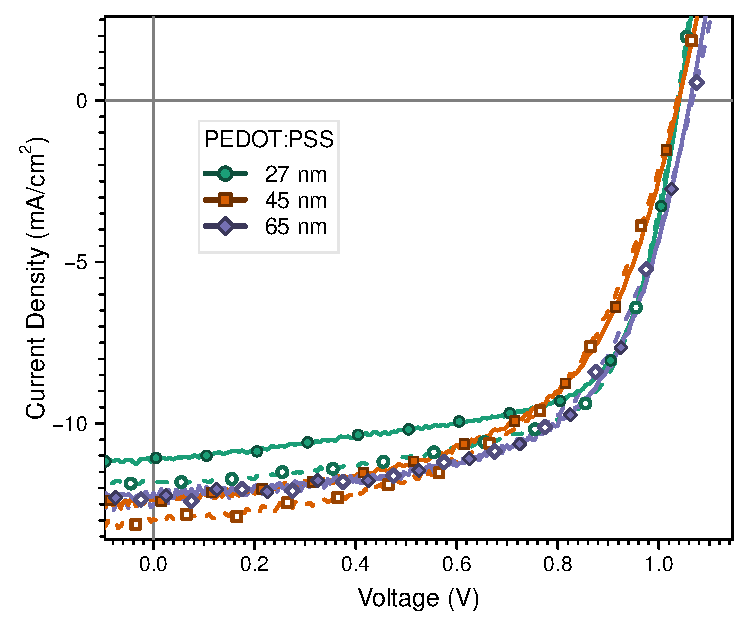
\includegraphics[width=0.8\textwidth]{jv_champions-pedotpss/pedotpss-IVs.pdf}
	\mycaption[Current-voltage sweeps for champion devices with different \glsentrytext{pedotpss} thicknesses.]{The solid line with filled markers represents the forward scan, while the dashed line with hollow markers represents the reverse scan.}\label{fig:thicknesses-jv_champions-pedotpss}
\end{SCfigure}

Using different spin coating speeds, devices with various \gls{pedotpss} thicknesses were obtained, as detailed in \cref{table:pedotpss_thickness}.
The \gls{ito} roughness is small enough to make us certain that even the thinner, \SI{27}{\nm}, \gls{pedotpss} layer results in an homogeneous coverage.

\paragraph{Current-voltage sweeps}
In \cref{fig:thicknesses-jv_champions-pedotpss} we can observe the current-voltage sweeps of the champion devices while in \cref{table:thicknesses_jv} the averages and standard deviations are reported.
None of the current\hyp{}voltage sweep parameters has shown a significant dependency on the \gls{pedotpss} \gls{htm} thickness.
Indeed, the high holes mobility of \gls{pedotpss} \cite{Rutledge2013} was expected to make this layer to be a non\hyp{}limiting one.


%\paragraph{Current-voltage sweeps -- \gls{ff}}
%The \gls{ff} is 
%
%\paragraph{Current-voltage sweeps -- \gls{voc}}
%
%\paragraph{Current-voltage sweeps -- \gls{jsc} and \gls{pce}}




\begin{figure}
	\makebox[\textwidth][c]{
		\parbox{1.1\textwidth}{
			\centering
			\begin{subfigure}[t]{0.51\textwidth}
				\includegraphics[width=1\textwidth]{photophysics-pedotpss/photophysics-CEs.pdf}
				\subcaption{Charge from \gls{ce}}\label{fig:thicknesses-pedotpss-geometric-ce}
			\end{subfigure}
			\qquad
			\begin{subfigure}[t]{0.51\textwidth}
				\includegraphics[width=1\textwidth]{photophysics-pedotpss/photophysics-DCs-capacitance.pdf}
				\subcaption{Capacitance from \gls{dc}}\label{fig:thicknesses-pedotpss-geometric-dc}
			\end{subfigure}
			\mycaption[CE and DC of devices with different \glsentrytext{pedotpss} thicknesses, highlighting the varying geometric capacitance.]{
				In (\textbf{a}) the charge \textsl{versus} light bias as obtained from \gls{ce} is reported. The dark solid line is an exponential fitting following \cref{eq:ce_full} while the light solid line reports just its exponential addend, ignoring the geometric capacitance. In (\textbf{b}) the capacitance dependence on light bias is reported as obtained from \gls{dc}. The solid line indicates the fitting using \cref{eq:dc_full}. All the fitted parameters are reported in \cref{table:thicknesses_photophysics}.
			}\label{fig:thicknesses-pedotpss-geometric}
		}
	}
\end{figure}

\paragraph{Geometric capacitance from \gls{dc} and \gls{ce}}
Changing the \gls{pedotpss} \gls{htm} layer thickness did not affect the measured geometric capacitance values reported in \cref{table:thicknesses_photophysics} and observable in \cref{fig:thicknesses-pedotpss-geometric}.
This can either mean that no charge accumulates close to the \gls{ito}\-/\gls{pedotpss} interface (\textsl{e.g.} in case the two materials have the same workfunction) or, considering the series of parallel plate capacitors model, that this layer's large capacitance does not influence the total measured capacitance.

\section{Series of CapacitorsAAAAAAAA}

As mentioned in the previous sections, the system can be thought as a series of three capacitors, each one including a different "dielectric".
From the tabulated values of relative permittivity of $\epsilon_|r|\approx3.9$ for \gls{pcbm70} \cite{Torabi2015} and the high frequency $\epsilon_|r|$ is from \SIrange{2.2}{2.6}{} for \gls{pedotpss} \cite{Rutledge2013,Yamashita2011}.



%\paragraph{Exponential charge distribution from \gls{dc} and \gls{ce}}

%\paragraph{Carriers life-time}
%
%\begin{figure}
%	\makebox[\textwidth][c]{
%		\parbox{1.1\textwidth}{
%			\centering
%			\begin{subfigure}[t]{0.51\textwidth}
%				\includegraphics[width=1\textwidth]{photophysics-pedotpss/photophysics-TPVCEs-nogeom_total.pdf}
%				\subcaption{\Gls{tpv} life-time \textsl{versus} \gls{ce} charge}\label{fig:thicknesses-pedotpss-tpv-ce}
%			\end{subfigure}
%			\qquad
%			\begin{subfigure}[t]{0.51\textwidth}
%				\includegraphics[width=1\textwidth]{photophysics-pedotpss/photophysics-TPVDCs-nogeom_total.pdf}
%				\subcaption{\Gls{tpv} life-time \textsl{versus} \gls{dc} charge}\label{fig:thicknesses-pedotpss-tpv-dc}
%			\end{subfigure}
%			\mycaption[Total carrier life-time \textsl{versus} charge of devices with different \glsentrytext{pedotpss} thicknesses.]{The small perturbation life-times were obtained \textsl{via} \gls{tpv} and corrected to total carrier life-time as reported in \cref{eq:tau_pfo}. In (\textbf{a}) the recombination orders needed for the correction were obtained from the fitting the small perturbation life-time \textsl{versus} chemical charge from \gls{ce}, while in (\textbf{b}) the chemical charge from \gls{dc} was used. Additionally, in (\textbf{a}) the chemical charge \textsl{versus} light bias needed for the $x$~axis, was taken from \gls{ce}, while in (\textbf{b}) it was obtained from \gls{dc}.}\label{fig:thicknesses-pedotpss-tpv}
%		}
%	}
%\end{figure}

\section{Conclusions}




